\documentclass[tikz,border=8pt]{standalone}
\usepackage{amsmath}
\usepackage{amssymb}
\usepackage{tikz}
\usetikzlibrary{arrows.meta,calc,decorations.pathreplacing,decorations.pathmorphing,patterns,shapes.geometric,positioning,shadings,plotmarks}

\begin{document}
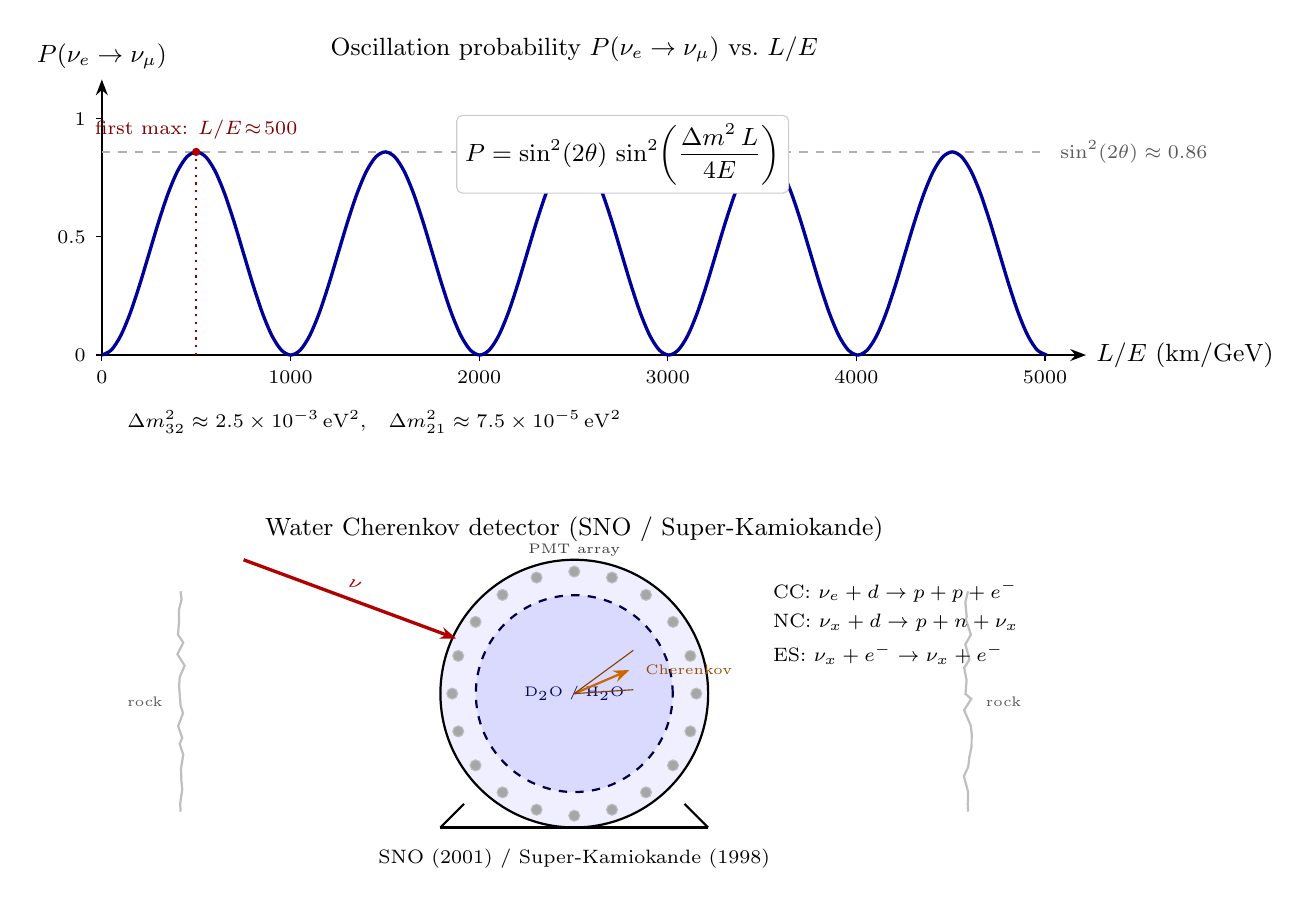
\begin{tikzpicture}[>={Stealth[length=2mm]}]

%% =====================================================================
%% TOP PANEL: Oscillation curve P(nu_e -> nu_mu) vs L/E
%% =====================================================================
\begin{scope}[shift={(0,5)}]
  % Plot frame: 12 cm wide axis, 3.0 cm tall plotting area.
  % L/E in [0, 5000] km/GeV  ->  x in [0, 12]   (scale: 12/5000 = 0.0024)
  % P   in [0, 1]            ->  y in [0, 3]    (scale: 3)

  % Title
  \node[anchor=south,font=\small] at (6,3.6) {Oscillation probability $P(\nu_e \to \nu_\mu)$ vs.\ $L/E$};

  % Axes
  \draw[->,thick] (0,0) -- (12.5,0) node[right,font=\small] {$L/E$ (km/GeV)};
  \draw[->,thick] (0,0) -- (0,3.5) node[above,font=\small] {$P(\nu_e\to\nu_\mu)$};

  % x-axis ticks at 0, 1000, 2000, 3000, 4000, 5000 km/GeV
  \foreach \xv/\xl in {0/0,1000/1000,2000/2000,3000/3000,4000/4000,5000/5000}{
    \pgfmathsetmacro{\xpos}{\xv*0.0024}
    \draw (\xpos,0) -- (\xpos,-0.08);
    \node[anchor=north,font=\scriptsize] at (\xpos,-0.08) {\xl};
  }

  % y-axis ticks at 0, 0.5, 1
  \foreach \yv/\yl in {0/0,0.5/0.5,1/1}{
    \pgfmathsetmacro{\ypos}{\yv*3}
    \draw (0,\ypos) -- (-0.08,\ypos);
    \node[anchor=east,font=\scriptsize] at (-0.08,\ypos) {\yl};
  }

  % Envelope amplitude sin^2(2theta) ~ 0.86 (y = 2.58)
  \draw[gray!60,dashed,thick] (0,2.58) -- (12,2.58);
  \node[anchor=west,font=\scriptsize,gray!70!black] at (12.05,2.58) {$\sin^2(2\theta) \approx 0.86$};

  % Oscillation curve: y = 3 * 0.86 * sin^2(pi * (L/E) / 1000)
  % First maximum at L/E = 500 km/GeV; period 1000 km/GeV.
  % Sampling step in L/E: 50 km/GeV (= 100 samples over 5000)
  \draw[blue!60!black,very thick]
    plot[smooth,samples=101,domain=0:12,variable=\u]
    ({\u},{3*0.86*(sin(180*\u/2.4))^2});

  % Mark first maximum at L/E = 500 km/GeV
  \pgfmathsetmacro{\xfm}{500*0.0024}
  \draw[red!60!black,dotted,thick] (\xfm,0) -- (\xfm,2.58);
  \fill[red!70!black] (\xfm,2.58) circle (1.5pt);
  \node[anchor=south,font=\scriptsize,red!50!black] at (\xfm,2.62)
    {first max: $L/E\!\approx\!500$};

  % Annotate the formula
  \node[anchor=north west,font=\small,fill=white,
        draw=gray!40,inner sep=3pt,rounded corners=2pt]
        at (4.5,3.05)
    {$P = \sin^2(2\theta)\,\sin^2\!\left(\dfrac{\Delta m^2\,L}{4E}\right)$};

  % Numerical values footnote
  \node[anchor=west,font=\scriptsize] at (0.2,-0.85)
    {$\Delta m_{32}^2 \approx 2.5\times 10^{-3}\,\mathrm{eV}^2$,\quad
     $\Delta m_{21}^2 \approx 7.5\times 10^{-5}\,\mathrm{eV}^2$};
\end{scope}

%% =====================================================================
%% BOTTOM PANEL: SNO/Super-K detector schematic
%% =====================================================================
\begin{scope}[shift={(0,-1.0)}]

  % Title
  \node[anchor=south,font=\small] at (6,3.5) {Water Cherenkov detector (SNO / Super-Kamiokande)};

  % Outer rocky cavern walls (suggestive)
  \draw[gray!50,thick,decorate,decoration={random steps,segment length=4pt,amplitude=1.5pt}]
    (1.0,0.2) -- (1.0,3.0);
  \draw[gray!50,thick,decorate,decoration={random steps,segment length=4pt,amplitude=1.5pt}]
    (11.0,0.2) -- (11.0,3.0);
  \node[font=\tiny,gray!70!black,anchor=west] at (0.2,1.6) {rock};
  \node[font=\tiny,gray!70!black,anchor=east] at (11.8,1.6) {rock};

  % Water shading
  \fill[blue!10,opacity=0.6] (6,1.7) circle (1.7);
  \fill[blue!20,opacity=0.6] (6,1.7) circle (1.25);

  % Outer stainless-steel tank
  \draw[black,thick] (6,1.7) circle (1.7);

  % Inner acrylic/SNO vessel
  \draw[blue!30!black,thick,dashed] (6,1.7) circle (1.25);

  % PMT array on inner wall of outer sphere
  \foreach \ang in {0,18,...,342}{
    \fill[gray!70] ({6+1.55*cos(\ang)},{1.7+1.55*sin(\ang)}) circle (0.07);
    \draw[gray!50,thin] ({6+1.55*cos(\ang)},{1.7+1.55*sin(\ang)}) circle (0.07);
  }

  % Inner labels
  \node[font=\tiny,blue!40!black] at (6,1.7) {D$_2$O / H$_2$O};
  \node[font=\tiny,gray!50!black,anchor=south] at (6,3.32) {PMT array};

  % Incoming neutrino arrow from upper left
  \draw[->,red!70!black,very thick] (1.8,3.4) -- (4.5,2.4)
    node[midway,above,sloped,font=\scriptsize] {$\nu$};

  % Reaction labels on right side
  \node[anchor=west,font=\scriptsize,align=left] at (8.4,3.0)
    {CC: $\nu_e + d \to p + p + e^-$};
  \node[anchor=west,font=\scriptsize,align=left] at (8.4,2.6)
    {NC: $\nu_x + d \to p + n + \nu_x$};
  \node[anchor=west,font=\scriptsize,align=left] at (8.4,2.2)
    {ES: $\nu_x + e^- \to \nu_x + e^-$};

  % Cherenkov cone illustration inside tank (small)
  \draw[orange!80!black,thick,->] (6,1.7) -- (6.7,2.0);
  \draw[orange!50!black,thin] (6,1.7) -- (6.75,2.25);
  \draw[orange!50!black,thin] (6,1.7) -- (6.75,1.75);
  \node[font=\tiny,orange!60!black,anchor=west] at (6.78,2.0) {Cherenkov};

  % Bottom support / base
  \draw[black,thick] (4.3,0) -- (7.7,0);
  \draw[black,thick] (4.3,0) -- (4.6,0.3);
  \draw[black,thick] (7.7,0) -- (7.4,0.3);

  % Caption inside
  \node[anchor=north,font=\scriptsize] at (6,-0.15)
    {SNO (2001) / Super-Kamiokande (1998)};

\end{scope}

\end{tikzpicture}
\end{document}
